\subsection{BP 6
  Solitary wave on a conical island (Laboratory)}

{\bf Documentation:}
\begin {itemize}


\item The Corps of Engineers website is the primary documentation for this benchmark problem:
\url{http://chl.erdc.usace.army.mil/chl.aspx?p=s&a=Projects;35}
\item A problem description is also provided by Frank Gonz\'alez 
 at \cite{bp-description}:\\
\href{https://github.com/rjleveque/nthmp-benchmark-problems/blob/master/BP06-FrankG-Solitary_wave_on_a_conical_island/Description.pdf}
{BP06-FrankG-Solitary\_wave\_on\_a\_conical\_island/Description.pdf} 
\item Numerous other publications also describe this experiment, in varying detail: \cite{SynolakisBernard:pmel135, Briggs1994, Liu1994, Briggs1995, Liu1995, Briggs1996, Fujima2000}
\end{itemize} 

\subsubsection{Description}
The goal of this Benchmark Problem (BP) is to compare computed model results with laboratory measurements obtained during a physical modeling experiment conducted at the Coastal and Hydraulic Laboratory, Engineer Research and Development Center of the U.S. Army Corps of Engineers.  The laboratory physical model was constructed as an idealized representation of Babi Island, in the Flores Sea, Indonesia, to compare with Babi Island runup measured shortly after the 12 December1992 Flores Island tsunami \cite{Yeh1994}.

\subsubsection {Problems encountered}

\begin {itemize}
\item Details of the laboratory setup and, therefore, the computational domain could not not be determined by the available documentation (above).  The version of the domain used in this report was developed after personal communication with Michael Briggs, U.S. Army Corps of Engineers, who  provided additional information on physical details of the laboratory experiment.  Unfortunately, it is not certain that accurate specification of details of the laboratory setup have been resolved.  In particular, the following items were not well documented and remain open to question: (a) the distance from the wavemaker face to the island center and (b) open gaps at each end of the wavemaker.
\item Erroneous entries were found in data files ts2a.txt, ts2b.txt and ts2cnew1.txt.  Several entries of the letter 'M' triggered read-in error messages; they were replaced by linear interpolation or extrapolation of neighboring values.
\item Initial values for some laboratory data were non-zero, rather than the zero values expected for initial wave basin conditions corresponding to still water. 
\end{itemize} 

\subsubsection{What we did}

\begin{itemize}
\item Used $g=9.81$ and no friction.
\item Used the computational domain presented in Figure \ref{bp6Domain}.

\item Used open boundary conditions for the top, bottom and right walls, and for the gaps between the ends of the wavemaker and the top and bottom walls.
\item Used inflow boundary conditions for the face of the wavemaker, as described in the Model Description section of this report.
\item Simulated Cases A and C, each with three different grid sizes and resolution, to demonstrate convergence:  28 X 24 (100 cm), 56 X 47 (50 cm) and  223 X 185 (12.5 cm)
\end{itemize}

\begin{figure}[ht]
\hfil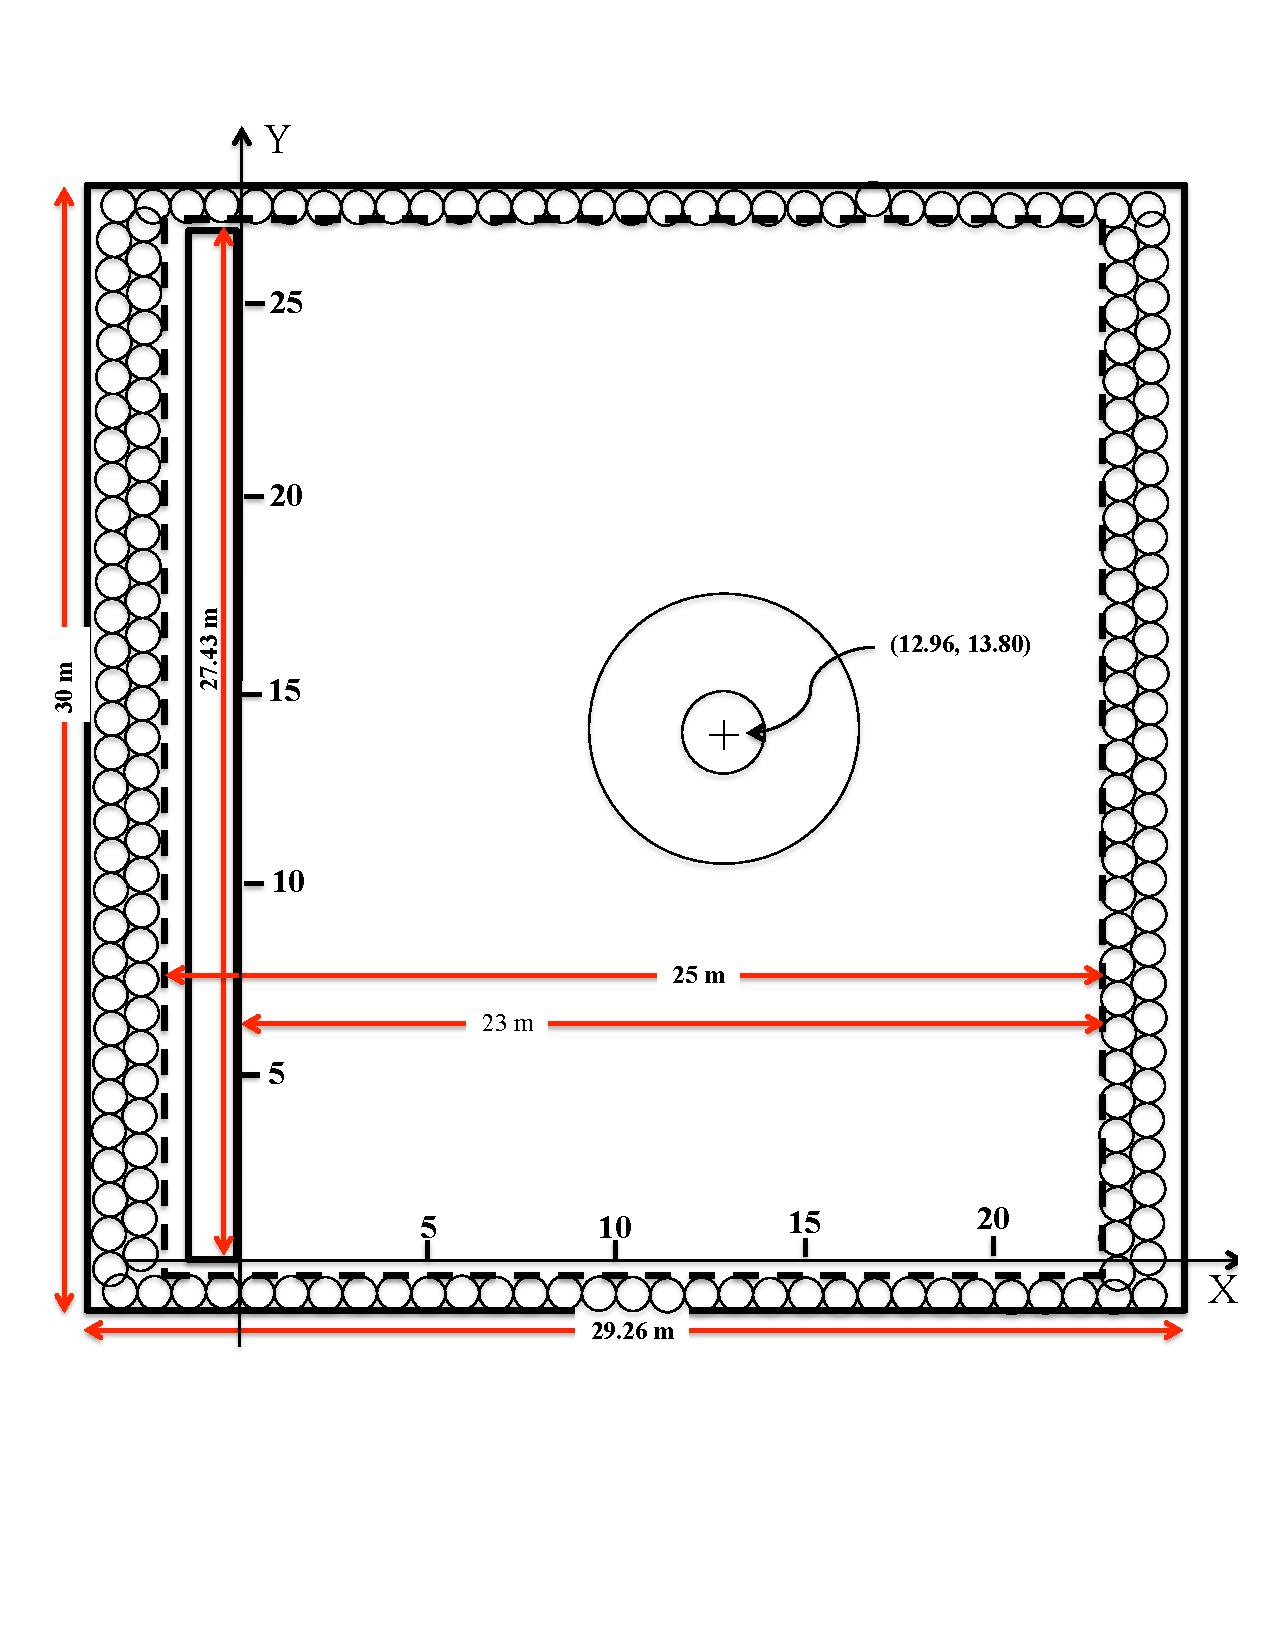
\includegraphics[width=6.0in]{bp6/Domain.pdf}\hfil
\caption{\label{bp6Domain}
Basin geometry and coordinate system.  Solid lines represent approximate basin and wavemaker vertical surfaces.  Circles along walls and dashed lines represent rolls of wave absorbing material.  Note the gaps of approximately 0.38 m between each end of the wavemaker and the adjacent wall.  Gage positions are given in Figure \ref{Table}.
  }
\end{figure}

\begin{figure}[ht]
\hfil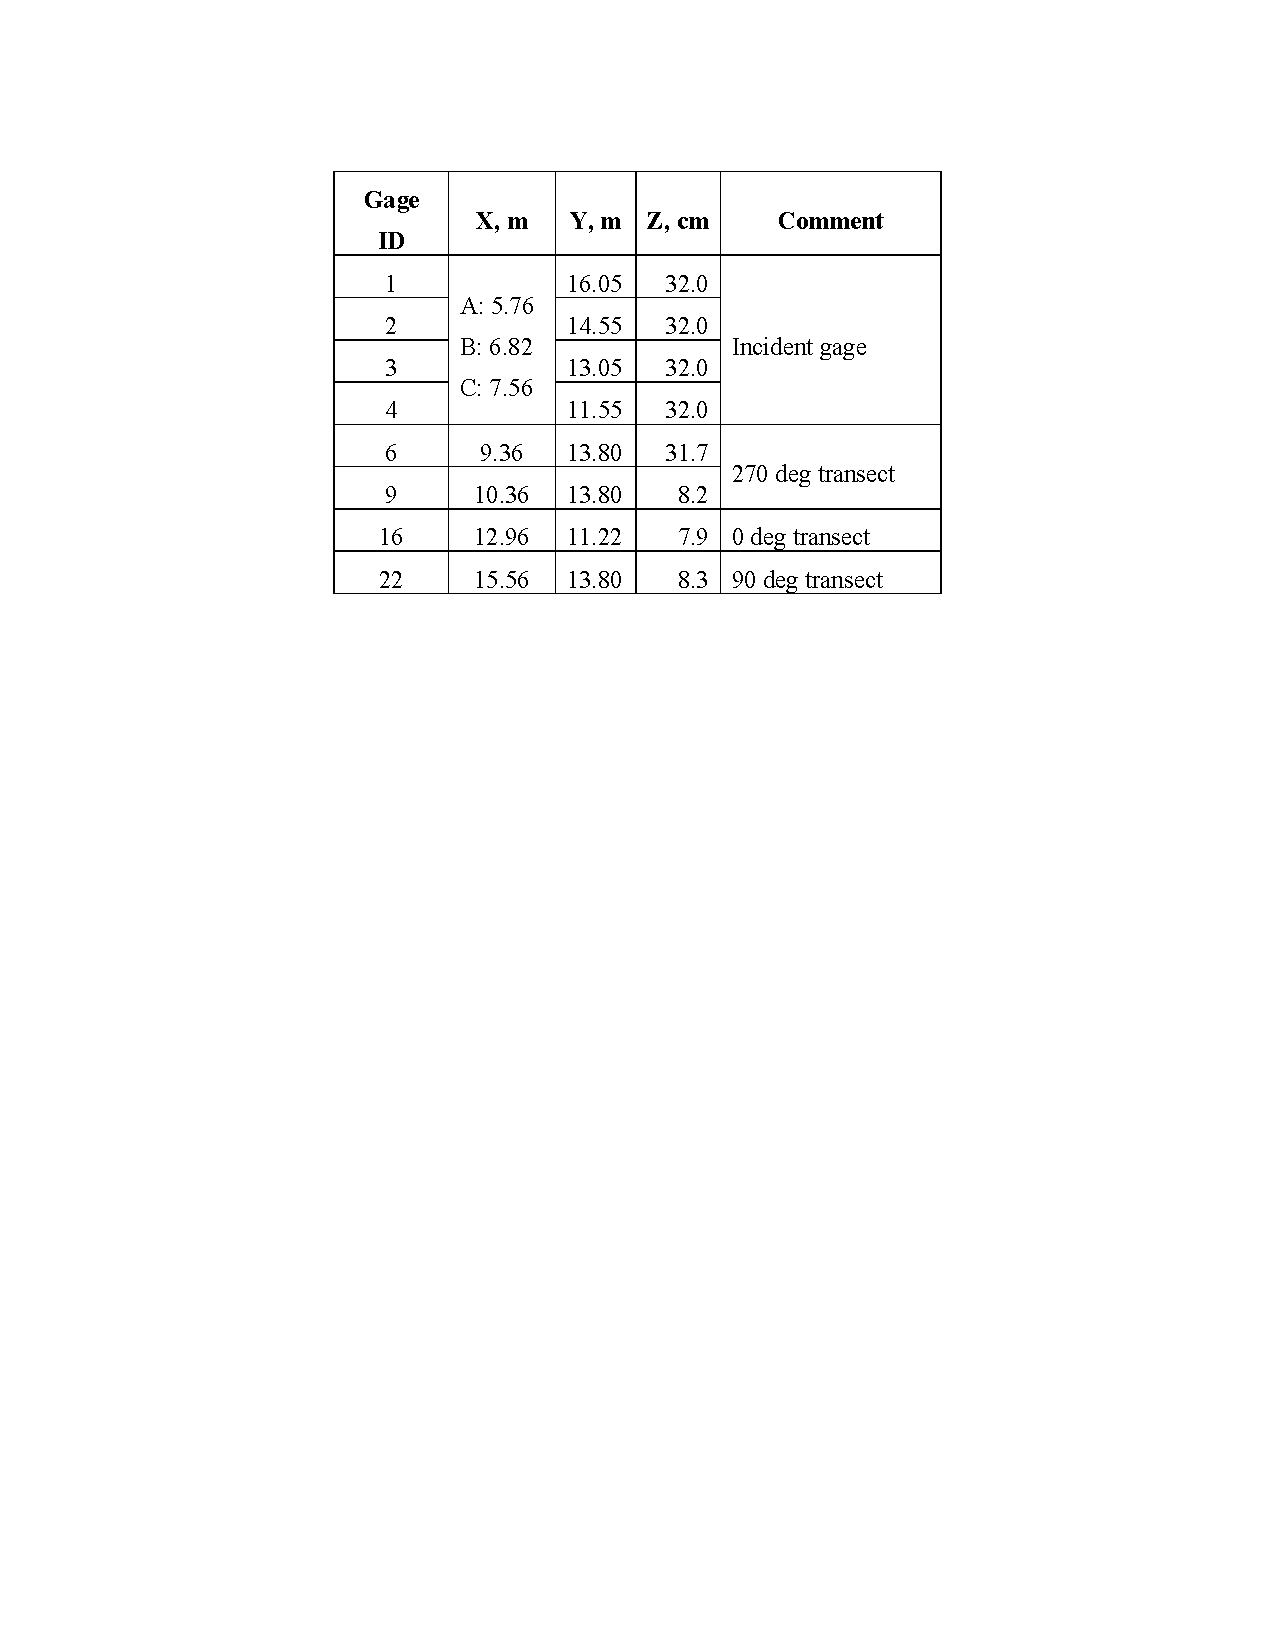
\includegraphics[width=5.0in]{bp6/Table.pdf}\hfil
\caption{\label{Table}
Coordinates of laboratory gauges 1, 2, 3, 4, 6, 9, 16, and 22.
  }
\end{figure} 

\subsubsection{Results}
  Requirements of this benchmark test were to:
\begin{itemize}
\item Demonstrate that two wave fronts split in front of the island and collide behind it
\item Demonstrate convergence of the solution as the computational grid is refined
\item Compare computed water level with laboratory data at gauges 1, 2, 3, 4, 6, 9, 16, and 22 (files ts2a.txt, ts2b.txt, ts2cnew1.txt)
\item Compare computed island runup with laboratory gage data (files run2a.txt, run2c.txt)
\end{itemize}

  The first benchmark requirement was satisfied, as seen in Figures \ref{A12-5Movie} and \ref{C12-5Movie}.  Thus, for Cases A \& C we see in frames t=30 to t=36 seconds that the initial wave splits into two wave fronts in front of the island, which then collide behind the island. 


  The second benchmark requirement was satisfied, as seen in Figures \ref{C100Gages}, \ref{C50Gages} and \ref{C12-5Gages}.  The agreement between Lab and GeoClaw time series is seen to improve as the computational grid resolution is decreased from 100 to 12.5 cm.  The most obvious manifestation of this convergence is the improved value of the first wave amplitude.

  The third benchmark requirement is satisfied by the comparisons presented in Figures \ref{A12-5Gages} and \ref{C12-5Gages}.  Good agreement is seen overall and, in particular, between computed and measured time series for the first wave.  The agreement for later wave details becomes progressively worse, as multiple reflections and refraction occur at the basin boundaries, the wavemaker face, and the island.  Note that in some cases, the laboratory gage data are characterized by non-zero initial values, which would be expected in the case of an initial condition corresponding to still water in the wave basin (see, e.g., gauge 2 for Cases A and C. 

  The final benchmark requirement is satisfied by the runup values presented in Figures \ref{A12-5Runup} and \ref{C12-5Runup}, in which good agreement is seen between the computed and measured runup on the conical island.

\subsubsection{Lessons learned}

\begin{itemize}
\item Accurate specification of the computational domain is essential, and every effort should be made to acquire this information.
\item Results demonstrate that the long wave equations are adequate to describe the major features of propagation, refraction and runup observed in the laboratory experiment.
\item Even with the unresolved details of the computational domain and lab data (i.e., non-zero initial values) the available data still provide a good benchmark test.
\end{itemize}

\begin{figure}[ht]
\hfil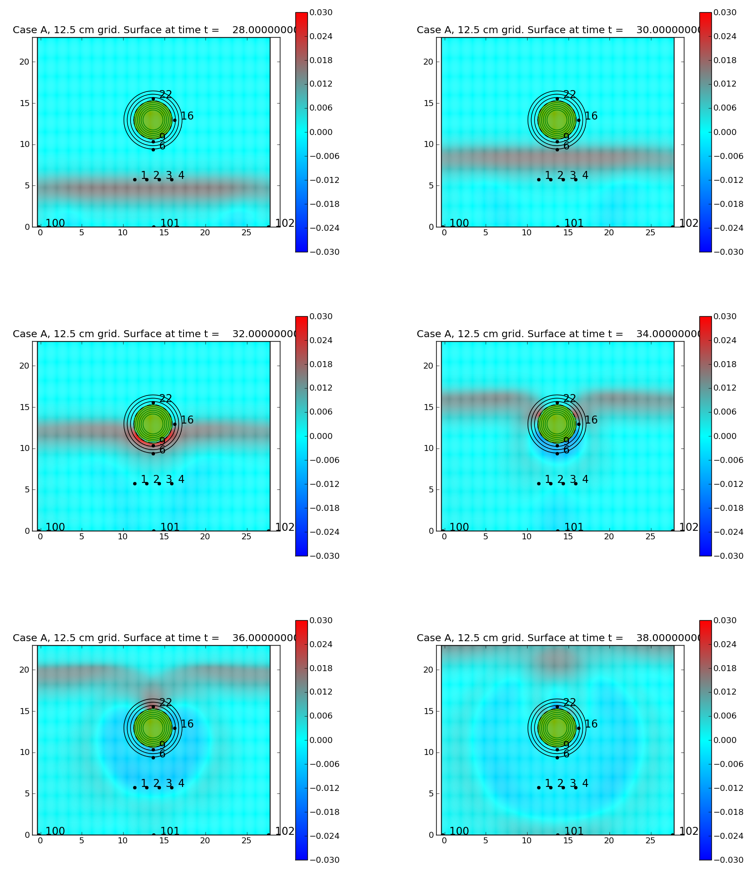
\includegraphics[width=7in]{bp6/A12-5Movie.png}\hfil
%\label{fig:A12-5Movie}
\caption{\label{A12-5Movie}
Animation snapshots of Case A for 12.5 cm resolution computational grid.
  }
\end{figure}

\begin{figure}[ht]
\hfil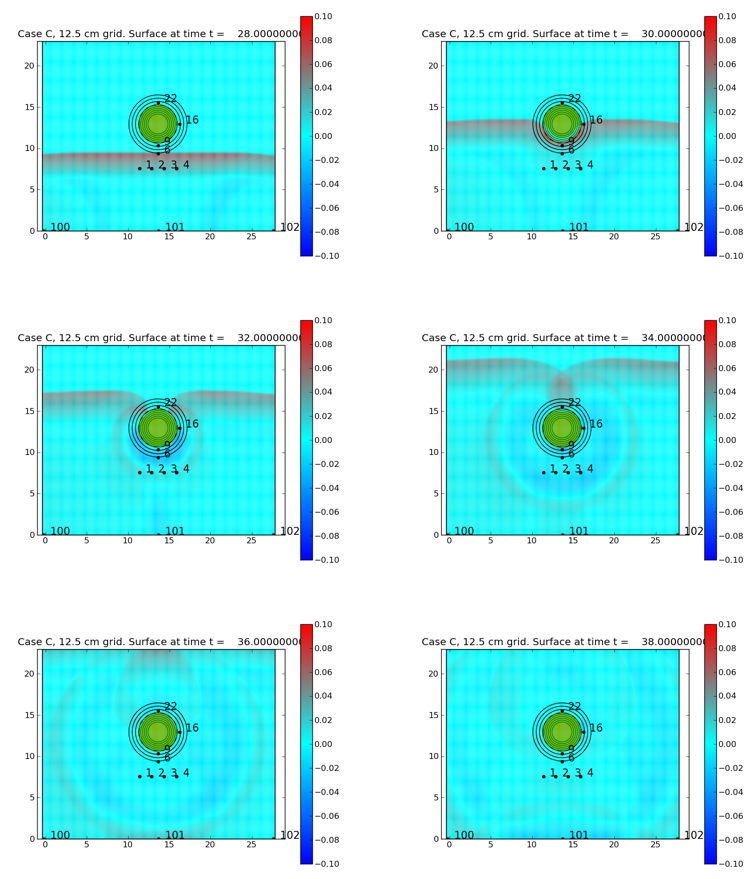
\includegraphics[width=7in]{bp6/C12-5Movie.png}\hfil
%\label{fig:C12-5Movie}
\caption{\label{C12-5Movie}
Animation snapshots of Case C for 12.5 cm resolution computational grid.
  }
\end{figure}

\begin{figure}[ht]
\hfil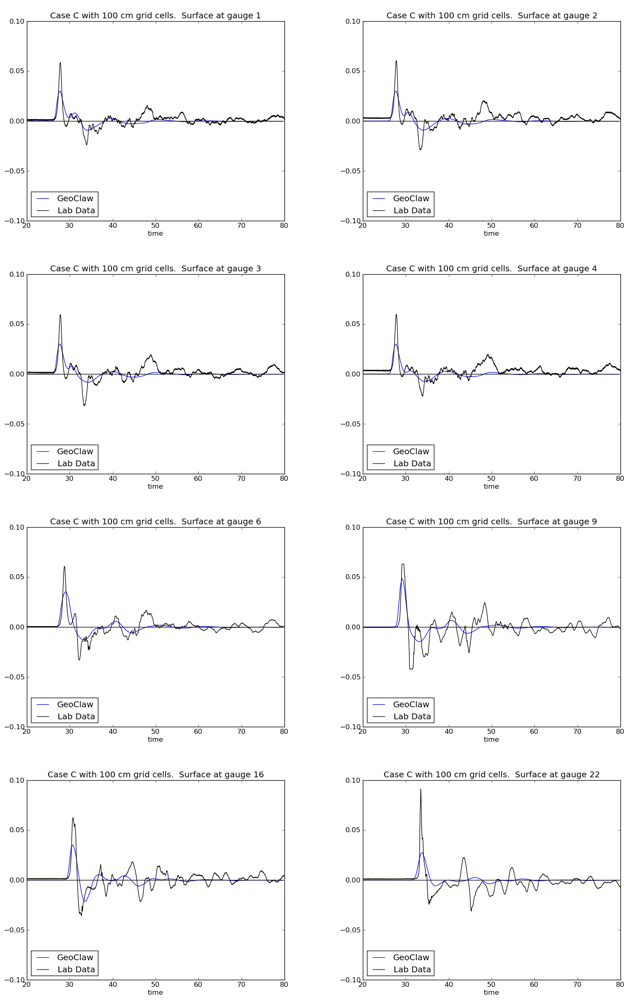
\includegraphics[height=8.5in]{bp6/C100Gages.png}\hfil
%\label{fig:C100Gages}
\caption{\label{C100Gages}
Comparison of laboratory gauge and GeoClaw time series for Case C, 100 cm resolution computational grid.
  }
\end{figure}

\begin{figure}[ht]
\hfil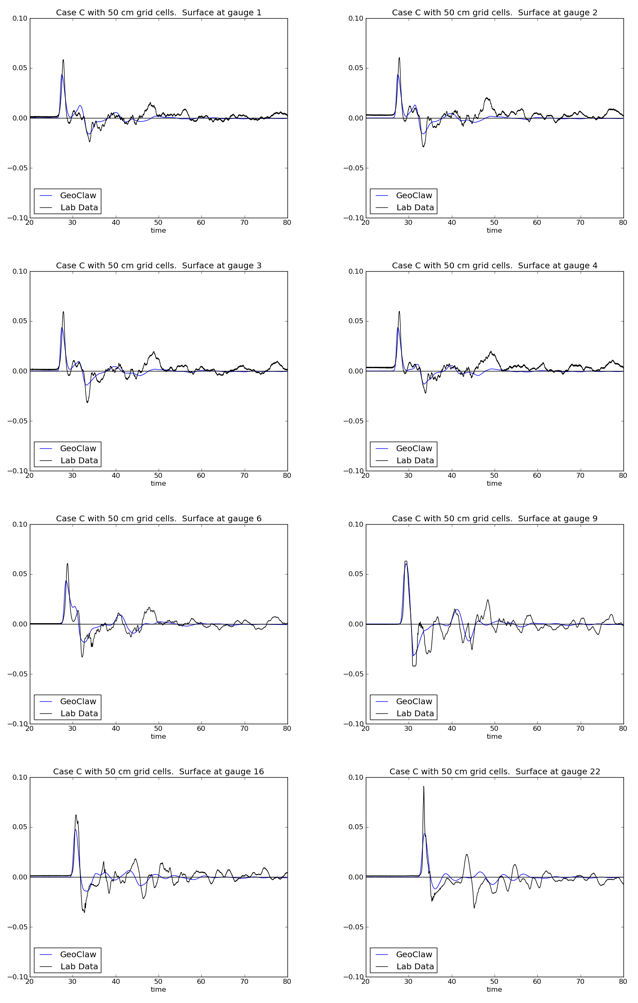
\includegraphics[height=8.5in]{bp6/C50Gages.png}\hfil
%\label{fig:C50Gages}
\caption{\label{C50Gages}
Comparison of laboratory gauge and GeoClaw time series for Case C, 50 cm resolution computational grid.
  }
\end{figure}

\begin{figure}[ht]
\hfil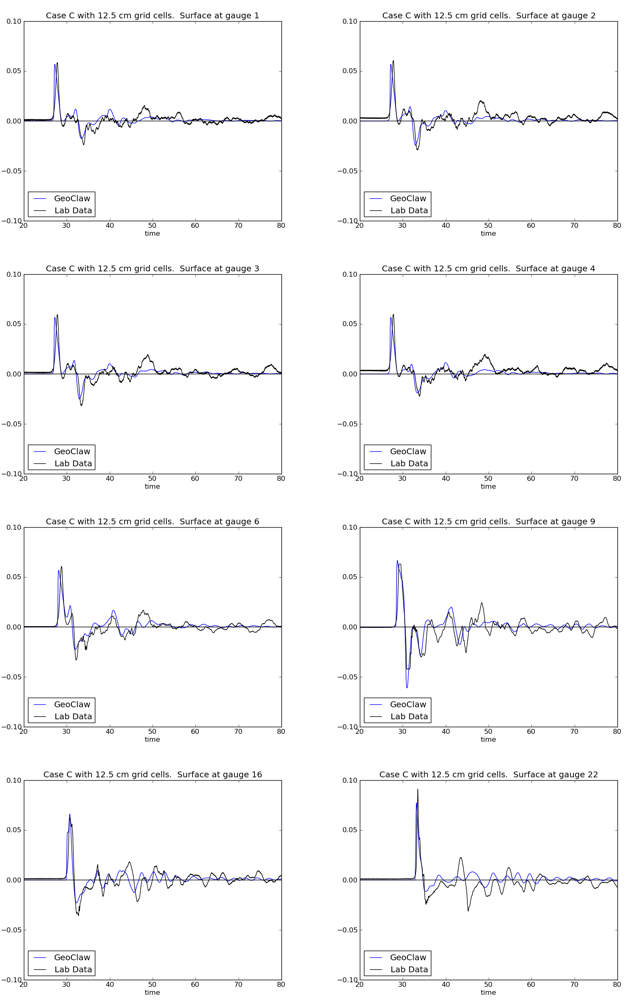
\includegraphics[height=8.5in]{bp6/C12-5Gages.png}\hfil
%\label{fig:C12-5Gages}
\caption{\label{C12-5Gages}
Comparison of laboratory gauge and GeoClaw time series for Case C, 12.5 cm resolution computational grid.
  }
\end{figure}


\begin{figure}[ht]
\hfil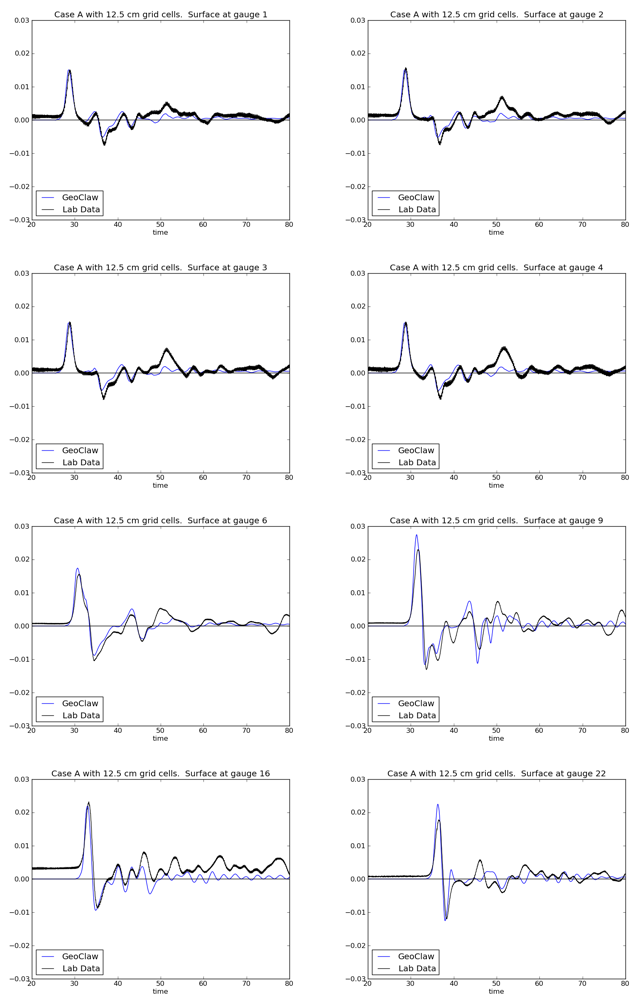
\includegraphics[height=8.5in]{bp6/A12-5Gages.png}\hfil
%\label{fig:A12-5Gages}
\caption{\label{A12-5Gages}
Comparison of laboratory gauge and GeoClaw time series for Case A, 12.5 cm resolution computational grid.
  }
\end{figure}

\begin{figure}[ht]
\hfil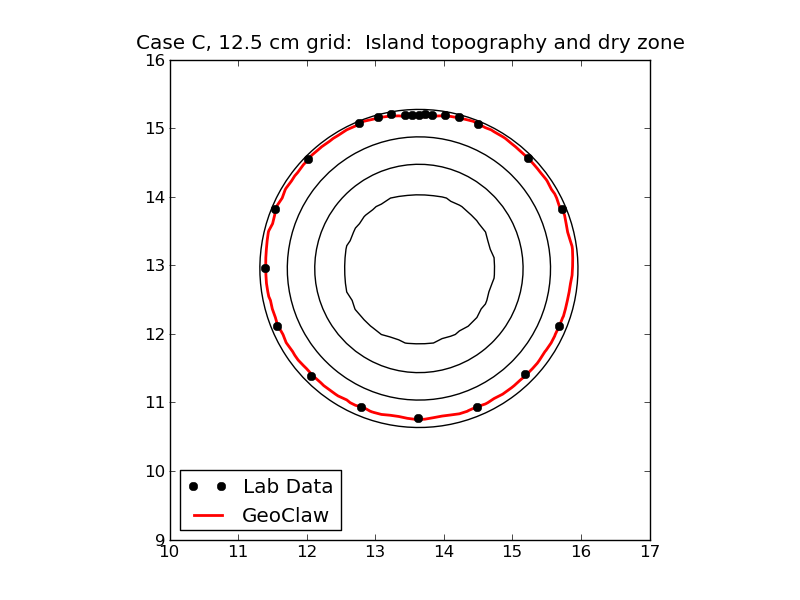
\includegraphics[width=5in]{bp6/A12-5Runup.png}\hfil
%\label{fig:A12-5Runup}
\caption{\label{A12-5Runup}
Island runup for Case A, using a 12.5 cm resolution computational grid.
  }
\end{figure}

\begin{figure}[ht]
\hfil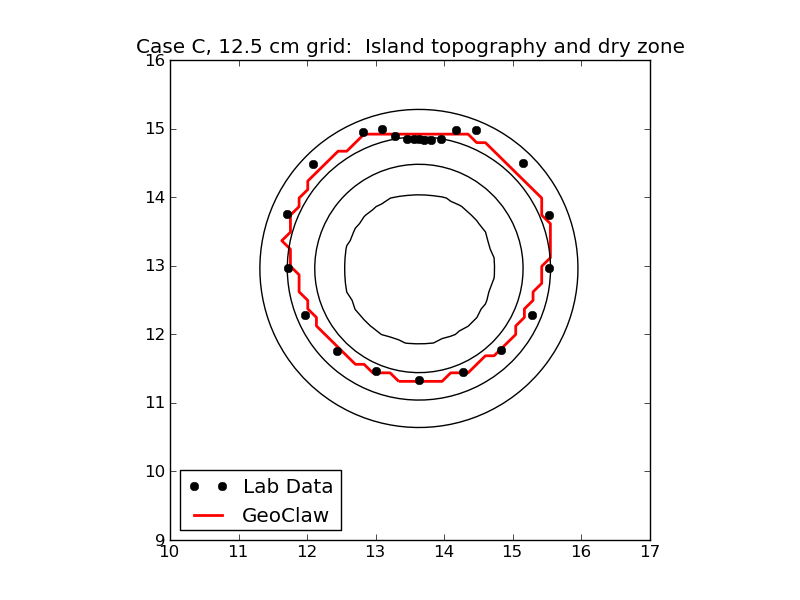
\includegraphics[width=5in]{bp6/C12-5Runup.png}\hfil
%\label{fig:C12-5Runup}
\caption{\label{C12-5Runup}
Island runup for Case C, using a 12.5 cm resolution computational grid.
  }
\end{figure}
